\documentclass[../main]{subfiles}

\begin{document}

\chapter{Methodology}
In the next chapter there will be the explaination of the data pipeline that the project followed.
In particular, each subsection will focus on a specific task, except for the data visualization that has been used only when needed.
% TODO: add references to Pandas an Numpy (?)

\section{Data Acquisition}
The used datasets are downloaded at runtime directly from the sources.
These datasets come directly from MovieLens' page and provides 6 different files.
More informations about the nature of the data are available \href{https://files.grouplens.org/datasets/movielens/ml-latest-README.html}{here}.
    \begin{table}[h]
        \center
        \begin{tabular}{|l | l|}
        \hline
        \textbf{Dataset} & \textbf{Features} \\
        \hline
        ratings.csv &  userId, movieId, rating, timestamp\\
        \hline
        tags.csv &  userId, movieId, tag, timestamp\\
        \hline
        movies.csv &  movieId, title, genres\\
        \hline
        links.csv &  movieId, imdbId, tmdbId\\
        \hline
        genome-scores.csv &  movieId, tagId, relevance\\
        \hline
        genome-tags.csv & tagId, tag\\
        \hline
        \end{tabular}
    \end{table}
        


Most of these datasets provides information for approximately 60000 films.
The links dataset provides two identifiers that allow to collect information from the IMDB and TMDB databases.
Thanks to the links' features, it has been possible to collect some more information on the running times of the films that could provide more insight into them.
Talking about the ground truth of the supervisioned models, the rating mean is missing. So the target feature will be computed during the pre-process phase thanks to the ratings dataset.
Further information about the features usage and the cardinality of the datasets will be discussed in the Pre-Process section.


\section{Data Pre-process}
In this section, will be discussed the pre-process phase for each of the above presented datasets.
In order to achieve a major clearity, the work on each dataset will be discussed in a specific subsection where the operation computed on them will be explained.
At the beginning of each subsection the cardinality will be reported.

\subsection*{Movies - movies.csv}
Cardinality: $58098 \times 3$

Inside this dataset, the title and generes features contains multiple information.
In particular, the title has been splitted in two part, where on one hand there's only the title name, and on the other, there's the year of the film production.
Since the title name is a string, that doesn't add more information to a classic machine learning model, this feature has been converted into its length meanwhile the production year just constitutes a new feature.
The genres feature contains a pipe separated list of a fixed possible values.
Since the list is just saying if a film has a specific genre or not, to each film, all the fixed values has been added as a feature, and if a genre appears into the genres feature, that column will result into 1 that indicate the presence of that genre, 0 otherwise.
At the end of this initial phase, the first sample of movies dataset looks like:
\begin{table}[h]
    \center
    \begin{tabular}{|c|c|c|c|c|c|c|c|}
    \hline
    \textbf{movieId} & \textbf{title\_len} & \textbf{year} & \textbf{action} & \textbf{adventure} & \textbf{\dots}  & \textbf{Western} & \textbf{(no genres listed)} \\
    \hline
    1                & 16                  & 1995          & 0               & 1                  & \dots           & 0                & 0                           \\
    \hline
    \end{tabular}
\end{table}

In order to finish the data pre-process on this dataset, the data cleaning is required.
First of all, there are some films where the year of the film production is missing.
Analyzing the distribuition of these, as showed in Figure \ref{fig:year_distribution_missing}, it is possible to see that the distribuition is right skewed, so the missing values can be filled with the \textbf{median}, as suggested during the lectures.
\begin{figure}[h]
    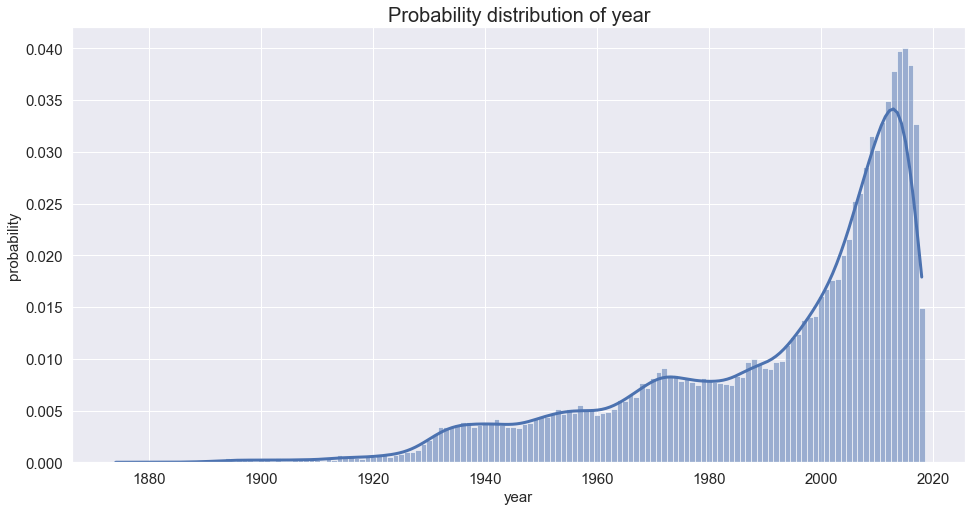
\includegraphics[width=\linewidth]{figures/year_distribution_missing.png}
    \caption{Right skewed probability distribution of the year feature}
    \label{fig:year_distribution_missing}
\end{figure}

Since the feature (no genres listed) and the films that has no genres provide no information about the film, they will be removed obtaining a final cardinality of $53832 \times 22$.

\subsection*{Tags - tags.csv}
Cardinality: $1108997 \times 4$

In order to use the relevant data from this dataset the timestamp and userId features have been deleted because they don't explain anything more about the films.
The information provided by each sample in the dataset are not very meaningful, for this reason it was decided to count the number of tags associated with each film, in order to understand how much interaction that film generated.
When a film doesn't have any related tag, the tag\_count can be setted to 0 because no users were interested on that film.
After these operations the cardinality was reduced to $45981 \times 2$.

\subsection*{Ratings - ratings.csv}
Cardinality: $27753443 \times 2$

The features in this dataset were necessary to find the target column.
In order to compute it, the average of each films' ratings has been calculated.
In addition, the number of the rating on each film has been counted.
However, the task of this project is the classification, for this reason the rating\_mean has been discretized in 10 bins, where each of them covers a rating range of 0.45 as showed in Figure \ref{fig:rating_mean_discretized}.

\begin{figure}[h]
    \center
    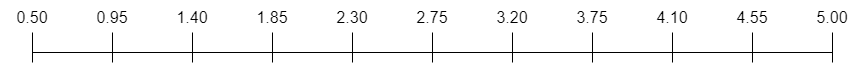
\includegraphics[width=\linewidth]{figures/step_rating_mean_discretized.png}
    \caption{Discretization of the rating\_mean feature}
    \label{fig:rating_mean_discretized}
\end{figure}

At the end, the final cardinality is $53889 \times 4$.

\subsection*{Genome - genome-scores.csv and genome-tags.csv}
Cardinality scores: $14862528 \times 3$

\noindent
Cardinality tags: $1128 \times 2$

Talking about these two datasets, the merge operation over the tagId was needed because it was interesting to associate the tagId with its string name.
After this union, on each sample there is the correspondence between a movieId, the tag name and the relevance of that tag.
The final step consist on relate every film to the relevance of each tag, using the pivot function, with the following result:
\begin{table}[h]
    \center
    \begin{tabular}{|c|c|c|c|c|c|c|c|}
    \hline
    \textbf{movieId} & \textbf{007}     & \textbf{18th century} & \textbf{action}  & \textbf{absurd} & \textbf{\dots} & \textbf{addiction} & \textbf{adventure} \\
    \hline
    1       & 0.02900 & 0.05425      & 0.66825 & 0.09725          & \dots & 0.07475   & 0.90700 \\
    \hline
    \end{tabular}
\end{table}

The final dataset named genome.csv has the cardinality equal to $13176 \times 1129$.

\subsection*{Links - links.csv}
Cardinality: $58098 \times 3$

On this dataset no pre-processing was needed because for each movie it contains two identifier that provide a link to external sources.
The interesting one is tmdbId because it has been used to retrieve information from the TMDB database.
Using the TMDB Api it has been possibile to build a new dataset that contains some additional features:
\begin{itemize}
    \item budget
    \item revenue
    \item adult
    \item runtime
\end{itemize}
In order to avoid the expensive operation of the Api calls, the resulted dataset has been saved in a GitHub \href{https://github.com/prushh/movie-lens-mlp/releases/tag/api-dataset}{release}.
Due to the insufficient amount of valid samples, the IMDb \href{https://datasets.imdbws.com/title.basics.tsv.gz}{title-basics.csv} dataset was downloaded to try to fill in all missing values.
After a brief exploration and analysis it has been possible to see that only the runtime feature has an enough amount of samples.
Since there continue to be some missing values, the distribution of this feature was analyzed in Figure \ref{fig:runtime_distribution_missing}.
It is possible to see that the distribuition is left skewed, so the missing values can be filled with the \textbf{median}.

\begin{figure}[h]
    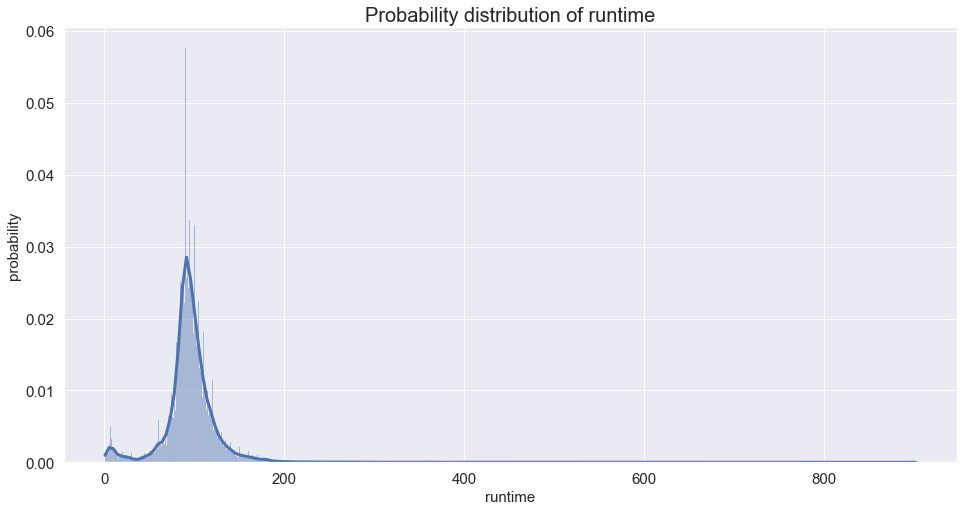
\includegraphics[width=\linewidth]{figures/runtime_distribution_missing.png}
    \caption{Left skewed probability distribution of the runtime feature}
    \label{fig:runtime_distribution_missing}
\end{figure}

The final cardinality of the acquired external resources is $58098 \times 2$.

\subsection*{Merged dataset}
In this section it will be showed how the cardinality of the used dataset has been created, starting from all the previously processed datasets.
In particular, the focus will be on the number of samples, because the number of features will increase by the addition of all the features in a single dataset.
Since, for a classification task, it is interesting to know the information about a sample, the starting dataset will be the movies one then all the other will be merged, trying to preserve the maximum number of samples.
The first merge has been between movies and ratings, because if a film doesn't have the target feature, it is useless to try to classify it. Moreover it has been discarded all the films that doesn't have a ratings means, obtaining a cardinality of: $50157 \times 24$.
The second merge is the one between the previously obtained dataset and tags, where there was an important number of samples that hasn't a tag count. In this case, these samples hasn't been discarded because they has been considered as the film didn't have generated any interaction from the users, so all the missing values has been filled with 0, obtaining the cardinality $50157 \times 25$ .
The third merge is between the previously generated dataset and the external resources. Since the external resources has a sample for each movie, the cardinality of this merge is $50157 \times 26$.
The final merge consider the genome dataset, where there is a big gap between the cardinality of this dataset, and the one that has build before. The choice on this merge was to discard all the data that didn't match with a sample on the genome dataset, because genome provides more and more interesting features with respect to the ones that the others dataset could provide. For this reason, the final cardinality of the dataset, after the merge operation is: $13147 \times 1154$
\subsection*{Data Transformation}

\section{Modeling}
\section{Performance Analysis}

\end{document}